\documentclass[1p]{elsarticle_modified}
%\bibliographystyle{elsarticle-num}

%\usepackage[colorlinks]{hyperref}
%\usepackage{abbrmath_seonhwa} %\Abb, \Ascr, \Acal ,\Abf, \Afrak
\usepackage{amsfonts}
\usepackage{amssymb}
\usepackage{amsmath}
\usepackage{amsthm}
\usepackage{scalefnt}
\usepackage{amsbsy}
\usepackage{kotex}
\usepackage{caption}
\usepackage{subfig}
\usepackage{color}
\usepackage{graphicx}
\usepackage{xcolor} %% white, black, red, green, blue, cyan, magenta, yellow
\usepackage{float}
\usepackage{setspace}
\usepackage{hyperref}

\usepackage{tikz}
\usetikzlibrary{arrows}

\usepackage{multirow}
\usepackage{array} % fixed length table
\usepackage{hhline}

%%%%%%%%%%%%%%%%%%%%%
\makeatletter
\renewcommand*\env@matrix[1][\arraystretch]{%
	\edef\arraystretch{#1}%
	\hskip -\arraycolsep
	\let\@ifnextchar\new@ifnextchar
	\array{*\c@MaxMatrixCols c}}
\makeatother %https://tex.stackexchange.com/questions/14071/how-can-i-increase-the-line-spacing-in-a-matrix
%%%%%%%%%%%%%%%

\usepackage[normalem]{ulem}

\newcommand{\msout}[1]{\ifmmode\text{\sout{\ensuremath{#1}}}\else\sout{#1}\fi}
%SOURCE: \msout is \stkout macro in https://tex.stackexchange.com/questions/20609/strikeout-in-math-mode

\newcommand{\cancel}[1]{
	\ifmmode
	{\color{red}\msout{#1}}
	\else
	{\color{red}\sout{#1}}
	\fi
}

\newcommand{\add}[1]{
	{\color{blue}\uwave{#1}}
}

\newcommand{\replace}[2]{
	\ifmmode
	{\color{red}\msout{#1}}{\color{blue}\uwave{#2}}
	\else
	{\color{red}\sout{#1}}{\color{blue}\uwave{#2}}
	\fi
}

\newcommand{\Sol}{\mathcal{S}} %segment
\newcommand{\D}{D} %diagram
\newcommand{\A}{\mathcal{A}} %arc


%%%%%%%%%%%%%%%%%%%%%%%%%%%%%5 test

\def\sl{\operatorname{\textup{SL}}(2,\Cbb)}
\def\psl{\operatorname{\textup{PSL}}(2,\Cbb)}
\def\quan{\mkern 1mu \triangleright \mkern 1mu}

\theoremstyle{definition}
\newtheorem{thm}{Theorem}[section]
\newtheorem{prop}[thm]{Proposition}
\newtheorem{lem}[thm]{Lemma}
\newtheorem{ques}[thm]{Question}
\newtheorem{cor}[thm]{Corollary}
\newtheorem{defn}[thm]{Definition}
\newtheorem{exam}[thm]{Example}
\newtheorem{rmk}[thm]{Remark}
\newtheorem{alg}[thm]{Algorithm}

\newcommand{\I}{\sqrt{-1}}
\begin{document}

%\begin{frontmatter}
%
%\title{Boundary parabolic representations of knots up to 8 crossings}
%
%%% Group authors per affiliation:
%\author{Yunhi Cho} 
%\address{Department of Mathematics, University of Seoul, Seoul, Korea}
%\ead{yhcho@uos.ac.kr}
%
%
%\author{Seonhwa Kim} %\fnref{s_kim}}
%\address{Center for Geometry and Physics, Institute for Basic Science, Pohang, 37673, Korea}
%\ead{ryeona17@ibs.re.kr}
%
%\author{Hyuk Kim}
%\address{Department of Mathematical Sciences, Seoul National University, Seoul 08826, Korea}
%\ead{hyukkim@snu.ac.kr}
%
%\author{Seokbeom Yoon}
%\address{Department of Mathematical Sciences, Seoul National University, Seoul, 08826,  Korea}
%\ead{sbyoon15@snu.ac.kr}
%
%\begin{abstract}
%We find all boundary parabolic representation of knots up to 8 crossings.
%
%\end{abstract}
%\begin{keyword}
%    \MSC[2010] 57M25 
%\end{keyword}
%
%\end{frontmatter}

%\linenumbers
%\tableofcontents
%
\newcommand\colored[1]{\textcolor{white}{\rule[-0.35ex]{0.8em}{1.4ex}}\kern-0.8em\color{red} #1}%
%\newcommand\colored[1]{\textcolor{white}{ #1}\kern-2.17ex	\textcolor{white}{ #1}\kern-1.81ex	\textcolor{white}{ #1}\kern-2.15ex\color{red}#1	}

{\Large $\underline{12a_{0018}~(K12a_{0018})}$}

\setlength{\tabcolsep}{10pt}
\renewcommand{\arraystretch}{1.6}
\vspace{1cm}\begin{tabular}{m{100pt}>{\centering\arraybackslash}m{274pt}}
\multirow{5}{120pt}{
	\centering
	\includegraphics[width=112pt]{../../../GIT/diagram.site/Diagrams/png/819_12a_0018.png}\\
\ \ \ A knot diagram\footnotemark}&
\allowdisplaybreaks
\textbf{Linearized knot diagam} \\
\cline{2-2}
 &
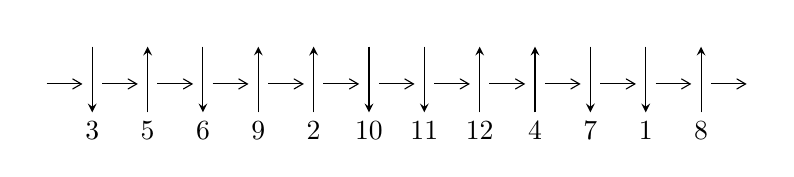
\begin{tikzpicture}[x=20pt, y=17pt]
	% nodes
	\node (C0) at (0, 0) {};
	\node (C1) at (1, 0) {};
	\node (C1U) at (1, +1) {};
	\node (C1D) at (1, -1) {3};

	\node (C2) at (2, 0) {};
	\node (C2U) at (2, +1) {};
	\node (C2D) at (2, -1) {5};

	\node (C3) at (3, 0) {};
	\node (C3U) at (3, +1) {};
	\node (C3D) at (3, -1) {6};

	\node (C4) at (4, 0) {};
	\node (C4U) at (4, +1) {};
	\node (C4D) at (4, -1) {9};

	\node (C5) at (5, 0) {};
	\node (C5U) at (5, +1) {};
	\node (C5D) at (5, -1) {2};

	\node (C6) at (6, 0) {};
	\node (C6U) at (6, +1) {};
	\node (C6D) at (6, -1) {10};

	\node (C7) at (7, 0) {};
	\node (C7U) at (7, +1) {};
	\node (C7D) at (7, -1) {11};

	\node (C8) at (8, 0) {};
	\node (C8U) at (8, +1) {};
	\node (C8D) at (8, -1) {12};

	\node (C9) at (9, 0) {};
	\node (C9U) at (9, +1) {};
	\node (C9D) at (9, -1) {4};

	\node (C10) at (10, 0) {};
	\node (C10U) at (10, +1) {};
	\node (C10D) at (10, -1) {7};

	\node (C11) at (11, 0) {};
	\node (C11U) at (11, +1) {};
	\node (C11D) at (11, -1) {1};

	\node (C12) at (12, 0) {};
	\node (C12U) at (12, +1) {};
	\node (C12D) at (12, -1) {8};
	\node (C13) at (13, 0) {};

	% arrows
	\draw[->,>={angle 60}]
	(C0) edge (C1) (C1) edge (C2) (C2) edge (C3) (C3) edge (C4) (C4) edge (C5) (C5) edge (C6) (C6) edge (C7) (C7) edge (C8) (C8) edge (C9) (C9) edge (C10) (C10) edge (C11) (C11) edge (C12) (C12) edge (C13) ;	\draw[->,>=stealth]
	(C1U) edge (C1D) (C2D) edge (C2U) (C3U) edge (C3D) (C4D) edge (C4U) (C5D) edge (C5U) (C6U) edge (C6D) (C7U) edge (C7D) (C8D) edge (C8U) (C9D) edge (C9U) (C10U) edge (C10D) (C11U) edge (C11D) (C12D) edge (C12U) ;
	\end{tikzpicture} \\
\hhline{~~} \\& 
\textbf{Solving Sequence} \\ \cline{2-2} 
 &
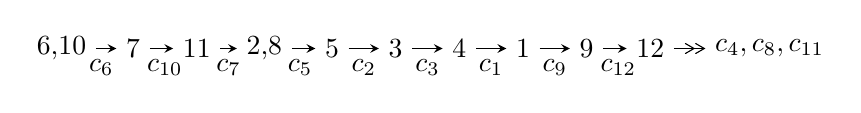
\begin{tikzpicture}[x=23pt, y=7pt]
	% node
	\node (A0) at (-1/8, 0) {6,10};
	\node (A1) at (1, 0) {7};
	\node (A2) at (2, 0) {11};
	\node (A3) at (49/16, 0) {2,8};
	\node (A4) at (33/8, 0) {5};
	\node (A5) at (41/8, 0) {3};
	\node (A6) at (49/8, 0) {4};
	\node (A7) at (57/8, 0) {1};
	\node (A8) at (65/8, 0) {9};
	\node (A9) at (73/8, 0) {12};
	\node (C1) at (1/2, -1) {$c_{6}$};
	\node (C2) at (3/2, -1) {$c_{10}$};
	\node (C3) at (5/2, -1) {$c_{7}$};
	\node (C4) at (29/8, -1) {$c_{5}$};
	\node (C5) at (37/8, -1) {$c_{2}$};
	\node (C6) at (45/8, -1) {$c_{3}$};
	\node (C7) at (53/8, -1) {$c_{1}$};
	\node (C8) at (61/8, -1) {$c_{9}$};
	\node (C9) at (69/8, -1) {$c_{12}$};
	\node (A10) at (11, 0) {$c_{4},c_{8},c_{11}$};

	% edge
	\draw[->,>=stealth]	
	(A0) edge (A1) (A1) edge (A2) (A2) edge (A3) (A3) edge (A4) (A4) edge (A5) (A5) edge (A6) (A6) edge (A7) (A7) edge (A8) (A8) edge (A9) ;
	\draw[->>,>={angle 60}]	
	(A9) edge (A10);
\end{tikzpicture} \\ 

\end{tabular} \\

\footnotetext{
The image of knot diagram is generated by the software ``\textbf{Draw programme}" developed by Andrew Bartholomew(\url{http://www.layer8.co.uk/maths/draw/index.htm\#Running-draw}), where we modified some parts for our purpose(\url{https://github.com/CATsTAILs/LinksPainter}).
}\phantom \\ \newline 
\centering \textbf{Ideals for irreducible components\footnotemark of $X_{\text{par}}$} 
 
\begin{align*}
I^u_{1}&=\langle 
-2.11930\times10^{181} u^{84}-3.51393\times10^{181} u^{83}+\cdots+4.67589\times10^{182} b-7.31431\times10^{181},\\
\phantom{I^u_{1}}&\phantom{= \langle  }-1.07455\times10^{183} u^{84}-2.39844\times10^{183} u^{83}+\cdots+6.82681\times10^{183} a+9.14213\times10^{183},\\
\phantom{I^u_{1}}&\phantom{= \langle  }u^{85}+3 u^{84}+\cdots-68 u+73\rangle \\
I^u_{2}&=\langle 
b- a-1,\;a^2+a+1,\;u^5+u^4-2 u^3- u^2+u-1\rangle \\
\\
\end{align*}
\raggedright * 2 irreducible components of $\dim_{\mathbb{C}}=0$, with total 95 representations.\\
\footnotetext{All coefficients of polynomials are rational numbers. But the coefficients are sometimes approximated in decimal forms when there is not enough margin.}
\newpage
\renewcommand{\arraystretch}{1}
\centering \section*{I. $I^u_{1}= \langle -2.12\times10^{181} u^{84}-3.51\times10^{181} u^{83}+\cdots+4.68\times10^{182} b-7.31\times10^{181},\;-1.07\times10^{183} u^{84}-2.40\times10^{183} u^{83}+\cdots+6.83\times10^{183} a+9.14\times10^{183},\;u^{85}+3 u^{84}+\cdots-68 u+73 \rangle$}
\flushleft \textbf{(i) Arc colorings}\\
\begin{tabular}{m{7pt} m{180pt} m{7pt} m{180pt} }
\flushright $a_{6}=$&$\begin{pmatrix}1\\0\end{pmatrix}$ \\
\flushright $a_{10}=$&$\begin{pmatrix}0\\u\end{pmatrix}$ \\
\flushright $a_{7}=$&$\begin{pmatrix}1\\u^2\end{pmatrix}$ \\
\flushright $a_{11}=$&$\begin{pmatrix}- u\\- u^3+u\end{pmatrix}$ \\
\flushright $a_{2}=$&$\begin{pmatrix}0.157402 u^{84}+0.351327 u^{83}+\cdots-11.2870 u-1.33915\\0.0453239 u^{84}+0.0751498 u^{83}+\cdots-5.90882 u+0.156426\end{pmatrix}$ \\
\flushright $a_{8}=$&$\begin{pmatrix}- u^2+1\\- u^4+2 u^2\end{pmatrix}$ \\
\flushright $a_{5}=$&$\begin{pmatrix}-0.0973095 u^{84}-0.243071 u^{83}+\cdots+12.7128 u+2.17784\\-0.0386728 u^{84}-0.0840276 u^{83}+\cdots+7.17860 u+1.28714\end{pmatrix}$ \\
\flushright $a_{3}=$&$\begin{pmatrix}0.108861 u^{84}+0.277515 u^{83}+\cdots+0.921763 u-2.89582\\0.0594798 u^{84}+0.134387 u^{83}+\cdots-4.79958 u-2.53940\end{pmatrix}$ \\
\flushright $a_{4}=$&$\begin{pmatrix}0.0493808 u^{84}+0.143127 u^{83}+\cdots+5.72134 u-0.356420\\0.0594798 u^{84}+0.134387 u^{83}+\cdots-4.79958 u-2.53940\end{pmatrix}$ \\
\flushright $a_{1}=$&$\begin{pmatrix}0.0447060 u^{84}+0.145350 u^{83}+\cdots-11.0547 u-5.38827\\-0.0550150 u^{84}-0.0997524 u^{83}+\cdots+2.36727 u-0.651555\end{pmatrix}$ \\
\flushright $a_{9}=$&$\begin{pmatrix}-0.00892540 u^{84}+0.0282388 u^{83}+\cdots+11.2989 u-1.76034\\-0.0540602 u^{84}-0.0446167 u^{83}+\cdots+2.04432 u-7.27963\end{pmatrix}$ \\
\flushright $a_{12}=$&$\begin{pmatrix}0.116080 u^{84}+0.273107 u^{83}+\cdots-17.9315 u-4.58050\\-0.0000810727 u^{84}-0.00974982 u^{83}+\cdots-2.36092 u+0.624367\end{pmatrix}$\\&\end{tabular}
\flushleft \textbf{(ii) Obstruction class $= -1$}\\~\\
\flushleft \textbf{(iii) Cusp Shapes $= -0.0954738 u^{84}-0.244184 u^{83}+\cdots-10.0507 u-7.23539$}\\~\\
\newpage\renewcommand{\arraystretch}{1}
\flushleft \textbf{(iv) u-Polynomials at the component}\newline \\
\begin{tabular}{m{50pt}|m{274pt}}
Crossings & \hspace{64pt}u-Polynomials at each crossing \\
\hline $$\begin{aligned}c_{1}\end{aligned}$$&$\begin{aligned}
&u^{85}+44 u^{84}+\cdots-7 u-1
\end{aligned}$\\
\hline $$\begin{aligned}c_{2},c_{5}\end{aligned}$$&$\begin{aligned}
&u^{85}+6 u^{84}+\cdots-7 u-1
\end{aligned}$\\
\hline $$\begin{aligned}c_{3}\end{aligned}$$&$\begin{aligned}
&u^{85}-6 u^{84}+\cdots+20709 u-4073
\end{aligned}$\\
\hline $$\begin{aligned}c_{4},c_{9}\end{aligned}$$&$\begin{aligned}
&u^{85}+u^{84}+\cdots+2048 u+1024
\end{aligned}$\\
\hline $$\begin{aligned}c_{6},c_{7},c_{10}\end{aligned}$$&$\begin{aligned}
&u^{85}+3 u^{84}+\cdots-68 u+73
\end{aligned}$\\
\hline $$\begin{aligned}c_{8},c_{12}\end{aligned}$$&$\begin{aligned}
&u^{85}-3 u^{84}+\cdots-2 u+1
\end{aligned}$\\
\hline $$\begin{aligned}c_{11}\end{aligned}$$&$\begin{aligned}
&u^{85}+49 u^{84}+\cdots-8 u-1
\end{aligned}$\\
\hline
\end{tabular}\\~\\
\newpage\renewcommand{\arraystretch}{1}
\flushleft \textbf{(v) Riley Polynomials at the component}\newline \\
\begin{tabular}{m{50pt}|m{274pt}}
Crossings & \hspace{64pt}Riley Polynomials at each crossing \\
\hline $$\begin{aligned}c_{1}\end{aligned}$$&$\begin{aligned}
&y^{85}+88 y^{83}+\cdots-31 y-1
\end{aligned}$\\
\hline $$\begin{aligned}c_{2},c_{5}\end{aligned}$$&$\begin{aligned}
&y^{85}+44 y^{84}+\cdots-7 y-1
\end{aligned}$\\
\hline $$\begin{aligned}c_{3}\end{aligned}$$&$\begin{aligned}
&y^{85}-44 y^{84}+\cdots-163840279 y-16589329
\end{aligned}$\\
\hline $$\begin{aligned}c_{4},c_{9}\end{aligned}$$&$\begin{aligned}
&y^{85}+55 y^{84}+\cdots-20971520 y-1048576
\end{aligned}$\\
\hline $$\begin{aligned}c_{6},c_{7},c_{10}\end{aligned}$$&$\begin{aligned}
&y^{85}-95 y^{84}+\cdots+44336 y-5329
\end{aligned}$\\
\hline $$\begin{aligned}c_{8},c_{12}\end{aligned}$$&$\begin{aligned}
&y^{85}+49 y^{84}+\cdots-8 y-1
\end{aligned}$\\
\hline $$\begin{aligned}c_{11}\end{aligned}$$&$\begin{aligned}
&y^{85}-23 y^{84}+\cdots-36 y-1
\end{aligned}$\\
\hline
\end{tabular}\\~\\
\newpage\flushleft \textbf{(vi) Complex Volumes and Cusp Shapes}
$$\begin{array}{c|c|c}  
\text{Solutions to }I^u_{1}& \I (\text{vol} + \sqrt{-1}CS) & \text{Cusp shape}\\
 \hline 
\begin{aligned}
u &= -0.073727 + 0.986667 I \\
a &= \phantom{-}0.936097 - 0.544165 I \\
b &= -0.476518 - 1.115450 I\end{aligned}
 & -2.14101 + 5.91470 I & \phantom{-0.000000 } 0 \\ \hline\begin{aligned}
u &= -0.073727 - 0.986667 I \\
a &= \phantom{-}0.936097 + 0.544165 I \\
b &= -0.476518 + 1.115450 I\end{aligned}
 & -2.14101 - 5.91470 I & \phantom{-0.000000 } 0 \\ \hline\begin{aligned}
u &= -0.664796 + 0.770883 I \\
a &= \phantom{-}1.38906 - 1.12816 I \\
b &= -0.517064 - 1.146120 I\end{aligned}
 & -3.42165 + 7.23133 I & \phantom{-0.000000 } 0 \\ \hline\begin{aligned}
u &= -0.664796 - 0.770883 I \\
a &= \phantom{-}1.38906 + 1.12816 I \\
b &= -0.517064 + 1.146120 I\end{aligned}
 & -3.42165 - 7.23133 I & \phantom{-0.000000 } 0 \\ \hline\begin{aligned}
u &= -0.319887 + 0.971190 I \\
a &= \phantom{-}0.524620 + 0.488014 I \\
b &= -0.441470 + 1.103310 I\end{aligned}
 & -2.42258 - 1.55579 I & \phantom{-0.000000 } 0 \\ \hline\begin{aligned}
u &= -0.319887 - 0.971190 I \\
a &= \phantom{-}0.524620 - 0.488014 I \\
b &= -0.441470 - 1.103310 I\end{aligned}
 & -2.42258 + 1.55579 I & \phantom{-0.000000 } 0 \\ \hline\begin{aligned}
u &= -0.849401 + 0.579207 I \\
a &= -0.146968 + 0.900614 I \\
b &= -0.360653 + 1.131480 I\end{aligned}
 & -4.52915 - 0.73034 I & \phantom{-0.000000 } 0 \\ \hline\begin{aligned}
u &= -0.849401 - 0.579207 I \\
a &= -0.146968 - 0.900614 I \\
b &= -0.360653 - 1.131480 I\end{aligned}
 & -4.52915 + 0.73034 I & \phantom{-0.000000 } 0 \\ \hline\begin{aligned}
u &= -0.810927 + 0.493483 I \\
a &= -0.86574 + 2.36356 I \\
b &= \phantom{-}0.493182 + 1.063790 I\end{aligned}
 & -2.34026 + 6.33705 I & \phantom{-0.000000 } 0 \\ \hline\begin{aligned}
u &= -0.810927 - 0.493483 I \\
a &= -0.86574 - 2.36356 I \\
b &= \phantom{-}0.493182 - 1.063790 I\end{aligned}
 & -2.34026 - 6.33705 I & \phantom{-0.000000 } 0\\
 \hline 
 \end{array}$$\newpage$$\begin{array}{c|c|c}  
\text{Solutions to }I^u_{1}& \I (\text{vol} + \sqrt{-1}CS) & \text{Cusp shape}\\
 \hline 
\begin{aligned}
u &= -0.607526 + 0.641631 I \\
a &= \phantom{-}0.329627 - 0.477034 I \\
b &= -0.707421 + 0.221133 I\end{aligned}
 & -0.75202 + 2.57285 I & \phantom{-0.000000 } 0 \\ \hline\begin{aligned}
u &= -0.607526 - 0.641631 I \\
a &= \phantom{-}0.329627 + 0.477034 I \\
b &= -0.707421 - 0.221133 I\end{aligned}
 & -0.75202 - 2.57285 I & \phantom{-0.000000 } 0 \\ \hline\begin{aligned}
u &= \phantom{-}0.680815 + 0.531192 I \\
a &= -0.475784 - 0.021071 I \\
b &= \phantom{-}0.656015 - 0.711309 I\end{aligned}
 & -0.52068 - 4.98776 I & \phantom{-0.000000 -}0. + 10.01892 I \\ \hline\begin{aligned}
u &= \phantom{-}0.680815 - 0.531192 I \\
a &= -0.475784 + 0.021071 I \\
b &= \phantom{-}0.656015 + 0.711309 I\end{aligned}
 & -0.52068 + 4.98776 I & \phantom{-0.000000 } 0. - 10.01892 I \\ \hline\begin{aligned}
u &= \phantom{-}0.947774 + 0.683916 I \\
a &= \phantom{-}0.056456 + 0.361169 I \\
b &= -0.766931 - 0.259594 I\end{aligned}
 & -2.68653 - 6.83343 I & \phantom{-0.000000 } 0 \\ \hline\begin{aligned}
u &= \phantom{-}0.947774 - 0.683916 I \\
a &= \phantom{-}0.056456 - 0.361169 I \\
b &= -0.766931 + 0.259594 I\end{aligned}
 & -2.68653 + 6.83343 I & \phantom{-0.000000 } 0 \\ \hline\begin{aligned}
u &= -0.612245 + 0.547885 I \\
a &= \phantom{-}0.732372 + 0.265000 I \\
b &= \phantom{-}0.473509 - 0.307517 I\end{aligned}
 & -0.28355 + 2.24163 I & \phantom{-0.000000 } 0. - 4.15869 I \\ \hline\begin{aligned}
u &= -0.612245 - 0.547885 I \\
a &= \phantom{-}0.732372 - 0.265000 I \\
b &= \phantom{-}0.473509 + 0.307517 I\end{aligned}
 & -0.28355 - 2.24163 I & \phantom{-0.000000 -}0. + 4.15869 I \\ \hline\begin{aligned}
u &= -0.426296 + 0.697949 I \\
a &= \phantom{-}0.918803 - 0.215162 I \\
b &= -0.272552 - 0.382600 I\end{aligned}
 & -0.09111 + 1.93411 I & \phantom{-0.000000 } 0. - 2.82382 I \\ \hline\begin{aligned}
u &= -0.426296 - 0.697949 I \\
a &= \phantom{-}0.918803 + 0.215162 I \\
b &= -0.272552 + 0.382600 I\end{aligned}
 & -0.09111 - 1.93411 I & \phantom{-0.000000 -}0. + 2.82382 I\\
 \hline 
 \end{array}$$\newpage$$\begin{array}{c|c|c}  
\text{Solutions to }I^u_{1}& \I (\text{vol} + \sqrt{-1}CS) & \text{Cusp shape}\\
 \hline 
\begin{aligned}
u &= -0.081024 + 0.790295 I \\
a &= \phantom{-}0.754750 - 0.090029 I \\
b &= -0.514454 + 0.225014 I\end{aligned}
 & \phantom{-}0.35550 + 1.80819 I & \phantom{-}1.92357 - 4.64833 I \\ \hline\begin{aligned}
u &= -0.081024 - 0.790295 I \\
a &= \phantom{-}0.754750 + 0.090029 I \\
b &= -0.514454 - 0.225014 I\end{aligned}
 & \phantom{-}0.35550 - 1.80819 I & \phantom{-}1.92357 + 4.64833 I \\ \hline\begin{aligned}
u &= -1.212560 + 0.159917 I \\
a &= \phantom{-}0.983042 - 0.860730 I \\
b &= -0.215414 - 0.748399 I\end{aligned}
 & -2.86425 + 1.08010 I & \phantom{-0.000000 } 0 \\ \hline\begin{aligned}
u &= -1.212560 - 0.159917 I \\
a &= \phantom{-}0.983042 + 0.860730 I \\
b &= -0.215414 + 0.748399 I\end{aligned}
 & -2.86425 - 1.08010 I & \phantom{-0.000000 } 0 \\ \hline\begin{aligned}
u &= \phantom{-}1.114220 + 0.566791 I \\
a &= -0.040385 - 1.282380 I \\
b &= -0.304170 - 1.134360 I\end{aligned}
 & -6.91731 - 3.67064 I & \phantom{-0.000000 } 0 \\ \hline\begin{aligned}
u &= \phantom{-}1.114220 - 0.566791 I \\
a &= -0.040385 + 1.282380 I \\
b &= -0.304170 + 1.134360 I\end{aligned}
 & -6.91731 + 3.67064 I & \phantom{-0.000000 } 0 \\ \hline\begin{aligned}
u &= \phantom{-}1.000140 + 0.768979 I \\
a &= \phantom{-}1.20857 + 1.42294 I \\
b &= -0.540479 + 1.152630 I\end{aligned}
 & -5.31540 - 11.73820 I & \phantom{-0.000000 } 0 \\ \hline\begin{aligned}
u &= \phantom{-}1.000140 - 0.768979 I \\
a &= \phantom{-}1.20857 - 1.42294 I \\
b &= -0.540479 - 1.152630 I\end{aligned}
 & -5.31540 + 11.73820 I & \phantom{-0.000000 } 0 \\ \hline\begin{aligned}
u &= \phantom{-}0.701004 + 0.167089 I \\
a &= -1.04043 - 0.96974 I \\
b &= -0.384455 - 1.189130 I\end{aligned}
 & -8.68594 + 3.54169 I & -10.91031 - 3.61355 I \\ \hline\begin{aligned}
u &= \phantom{-}0.701004 - 0.167089 I \\
a &= -1.04043 + 0.96974 I \\
b &= -0.384455 + 1.189130 I\end{aligned}
 & -8.68594 - 3.54169 I & -10.91031 + 3.61355 I\\
 \hline 
 \end{array}$$\newpage$$\begin{array}{c|c|c}  
\text{Solutions to }I^u_{1}& \I (\text{vol} + \sqrt{-1}CS) & \text{Cusp shape}\\
 \hline 
\begin{aligned}
u &= \phantom{-}0.566939 + 0.421860 I \\
a &= -1.063890 + 0.895906 I \\
b &= \phantom{-}0.625120 + 0.883968 I\end{aligned}
 & -1.019110 - 0.019860 I & -7.10656 + 3.63163 I \\ \hline\begin{aligned}
u &= \phantom{-}0.566939 - 0.421860 I \\
a &= -1.063890 - 0.895906 I \\
b &= \phantom{-}0.625120 - 0.883968 I\end{aligned}
 & -1.019110 + 0.019860 I & -7.10656 - 3.63163 I \\ \hline\begin{aligned}
u &= \phantom{-}1.324570 + 0.153827 I \\
a &= \phantom{-}0.888954 - 1.043400 I \\
b &= -0.219128 - 0.834236 I\end{aligned}
 & -6.48791 - 3.11039 I & \phantom{-0.000000 } 0 \\ \hline\begin{aligned}
u &= \phantom{-}1.324570 - 0.153827 I \\
a &= \phantom{-}0.888954 + 1.043400 I \\
b &= -0.219128 + 0.834236 I\end{aligned}
 & -6.48791 + 3.11039 I & \phantom{-0.000000 } 0 \\ \hline\begin{aligned}
u &= -0.629066 + 0.209720 I \\
a &= -0.61598 - 3.22202 I \\
b &= \phantom{-}0.372593 - 1.046640 I\end{aligned}
 & -3.20124 - 0.40319 I & -7.42049 + 0.02513 I \\ \hline\begin{aligned}
u &= -0.629066 - 0.209720 I \\
a &= -0.61598 + 3.22202 I \\
b &= \phantom{-}0.372593 + 1.046640 I\end{aligned}
 & -3.20124 + 0.40319 I & -7.42049 - 0.02513 I \\ \hline\begin{aligned}
u &= \phantom{-}0.162545 + 0.544040 I \\
a &= \phantom{-}0.451845 - 0.799524 I \\
b &= \phantom{-}0.472309 + 0.536803 I\end{aligned}
 & \phantom{-}0.99323 + 1.21291 I & \phantom{-}4.59661 - 3.40071 I \\ \hline\begin{aligned}
u &= \phantom{-}0.162545 - 0.544040 I \\
a &= \phantom{-}0.451845 + 0.799524 I \\
b &= \phantom{-}0.472309 - 0.536803 I\end{aligned}
 & \phantom{-}0.99323 - 1.21291 I & \phantom{-}4.59661 + 3.40071 I \\ \hline\begin{aligned}
u &= -1.45267\phantom{ +0.000000I} \\
a &= \phantom{-}0.691122\phantom{ +0.000000I} \\
b &= \phantom{-}0.654332\phantom{ +0.000000I}\end{aligned}
 & -3.81338\phantom{ +0.000000I} & \phantom{-0.000000 } 0 \\ \hline\begin{aligned}
u &= -0.191578 + 0.506538 I \\
a &= -0.351792 - 0.699095 I \\
b &= \phantom{-}0.549301 + 0.652031 I\end{aligned}
 & \phantom{-}0.95141 + 1.54224 I & \phantom{-}3.64572 - 4.77993 I\\
 \hline 
 \end{array}$$\newpage$$\begin{array}{c|c|c}  
\text{Solutions to }I^u_{1}& \I (\text{vol} + \sqrt{-1}CS) & \text{Cusp shape}\\
 \hline 
\begin{aligned}
u &= -0.191578 - 0.506538 I \\
a &= -0.351792 + 0.699095 I \\
b &= \phantom{-}0.549301 - 0.652031 I\end{aligned}
 & \phantom{-}0.95141 - 1.54224 I & \phantom{-}3.64572 + 4.77993 I \\ \hline\begin{aligned}
u &= \phantom{-}0.524049 + 0.111794 I \\
a &= -0.076692 + 1.324640 I \\
b &= -0.776293 - 0.119585 I\end{aligned}
 & -4.80858 - 0.38289 I & -6.98989 - 0.09954 I \\ \hline\begin{aligned}
u &= \phantom{-}0.524049 - 0.111794 I \\
a &= -0.076692 - 1.324640 I \\
b &= -0.776293 + 0.119585 I\end{aligned}
 & -4.80858 + 0.38289 I & -6.98989 + 0.09954 I \\ \hline\begin{aligned}
u &= \phantom{-}0.475918 + 0.244964 I \\
a &= \phantom{-}2.65951 + 1.54249 I \\
b &= -0.495221 + 1.182570 I\end{aligned}
 & -7.91886 - 5.05331 I & -9.98522 + 3.52204 I \\ \hline\begin{aligned}
u &= \phantom{-}0.475918 - 0.244964 I \\
a &= \phantom{-}2.65951 - 1.54249 I \\
b &= -0.495221 - 1.182570 I\end{aligned}
 & -7.91886 + 5.05331 I & -9.98522 - 3.52204 I \\ \hline\begin{aligned}
u &= \phantom{-}1.47833 + 0.03589 I \\
a &= -0.405383 - 0.632644 I \\
b &= \phantom{-}0.744958 - 0.816857 I\end{aligned}
 & -4.46882 - 2.78743 I & \phantom{-0.000000 } 0 \\ \hline\begin{aligned}
u &= \phantom{-}1.47833 - 0.03589 I \\
a &= -0.405383 + 0.632644 I \\
b &= \phantom{-}0.744958 + 0.816857 I\end{aligned}
 & -4.46882 + 2.78743 I & \phantom{-0.000000 } 0 \\ \hline\begin{aligned}
u &= \phantom{-}0.408053 + 0.323773 I \\
a &= -1.44582 - 2.40333 I \\
b &= \phantom{-}0.478977 - 0.992998 I\end{aligned}
 & -0.32720 - 2.78409 I & \phantom{-}1.83631 + 3.63493 I \\ \hline\begin{aligned}
u &= \phantom{-}0.408053 - 0.323773 I \\
a &= -1.44582 + 2.40333 I \\
b &= \phantom{-}0.478977 + 0.992998 I\end{aligned}
 & -0.32720 + 2.78409 I & \phantom{-}1.83631 - 3.63493 I \\ \hline\begin{aligned}
u &= \phantom{-}1.45414 + 0.29131 I \\
a &= \phantom{-}0.852958 + 0.820806 I \\
b &= -0.278597 + 0.750241 I\end{aligned}
 & -6.17711 - 5.61767 I & \phantom{-0.000000 } 0\\
 \hline 
 \end{array}$$\newpage$$\begin{array}{c|c|c}  
\text{Solutions to }I^u_{1}& \I (\text{vol} + \sqrt{-1}CS) & \text{Cusp shape}\\
 \hline 
\begin{aligned}
u &= \phantom{-}1.45414 - 0.29131 I \\
a &= \phantom{-}0.852958 - 0.820806 I \\
b &= -0.278597 - 0.750241 I\end{aligned}
 & -6.17711 + 5.61767 I & \phantom{-0.000000 } 0 \\ \hline\begin{aligned}
u &= \phantom{-}0.022495 + 0.486505 I \\
a &= -1.48819 - 1.58315 I \\
b &= \phantom{-}0.545824 - 0.945362 I\end{aligned}
 & \phantom{-}0.07724 - 2.86484 I & \phantom{-}1.199969 - 0.242830 I \\ \hline\begin{aligned}
u &= \phantom{-}0.022495 - 0.486505 I \\
a &= -1.48819 + 1.58315 I \\
b &= \phantom{-}0.545824 + 0.945362 I\end{aligned}
 & \phantom{-}0.07724 + 2.86484 I & \phantom{-}1.199969 + 0.242830 I \\ \hline\begin{aligned}
u &= -1.53385 + 0.07020 I \\
a &= -0.40293 + 2.49379 I \\
b &= \phantom{-}0.449202 + 1.155340 I\end{aligned}
 & -6.96879 + 4.07852 I & \phantom{-0.000000 } 0 \\ \hline\begin{aligned}
u &= -1.53385 - 0.07020 I \\
a &= -0.40293 - 2.49379 I \\
b &= \phantom{-}0.449202 - 1.155340 I\end{aligned}
 & -6.96879 - 4.07852 I & \phantom{-0.000000 } 0 \\ \hline\begin{aligned}
u &= -1.55923 + 0.08103 I \\
a &= \phantom{-}0.92915 - 2.02619 I \\
b &= -0.566136 - 1.204640 I\end{aligned}
 & -14.9606 + 6.2710 I & \phantom{-0.000000 } 0 \\ \hline\begin{aligned}
u &= -1.55923 - 0.08103 I \\
a &= \phantom{-}0.92915 + 2.02619 I \\
b &= -0.566136 + 1.204640 I\end{aligned}
 & -14.9606 - 6.2710 I & \phantom{-0.000000 } 0 \\ \hline\begin{aligned}
u &= -1.56350 + 0.03748 I \\
a &= -0.427946 - 0.305316 I \\
b &= -0.892662 + 0.229621 I\end{aligned}
 & -12.01330 + 0.94589 I & \phantom{-0.000000 } 0 \\ \hline\begin{aligned}
u &= -1.56350 - 0.03748 I \\
a &= -0.427946 + 0.305316 I \\
b &= -0.892662 - 0.229621 I\end{aligned}
 & -12.01330 - 0.94589 I & \phantom{-0.000000 } 0 \\ \hline\begin{aligned}
u &= -1.56534 + 0.10799 I \\
a &= -0.397551 - 0.704235 I \\
b &= \phantom{-}0.751803 - 0.834148 I\end{aligned}
 & -8.23473 + 1.87606 I & \phantom{-0.000000 } 0\\
 \hline 
 \end{array}$$\newpage$$\begin{array}{c|c|c}  
\text{Solutions to }I^u_{1}& \I (\text{vol} + \sqrt{-1}CS) & \text{Cusp shape}\\
 \hline 
\begin{aligned}
u &= -1.56534 - 0.10799 I \\
a &= -0.397551 + 0.704235 I \\
b &= \phantom{-}0.751803 + 0.834148 I\end{aligned}
 & -8.23473 - 1.87606 I & \phantom{-0.000000 } 0 \\ \hline\begin{aligned}
u &= \phantom{-}1.56363 + 0.14005 I \\
a &= \phantom{-}0.681046 - 0.008951 I \\
b &= \phantom{-}0.682539 + 0.031873 I\end{aligned}
 & -7.51475 - 4.66932 I & \phantom{-0.000000 } 0 \\ \hline\begin{aligned}
u &= \phantom{-}1.56363 - 0.14005 I \\
a &= \phantom{-}0.681046 + 0.008951 I \\
b &= \phantom{-}0.682539 - 0.031873 I\end{aligned}
 & -7.51475 + 4.66932 I & \phantom{-0.000000 } 0 \\ \hline\begin{aligned}
u &= \phantom{-}1.56682 + 0.18662 I \\
a &= -0.369496 + 0.287964 I \\
b &= -0.882048 - 0.243919 I\end{aligned}
 & -7.97573 - 5.57692 I & \phantom{-0.000000 } 0 \\ \hline\begin{aligned}
u &= \phantom{-}1.56682 - 0.18662 I \\
a &= -0.369496 - 0.287964 I \\
b &= -0.882048 + 0.243919 I\end{aligned}
 & -7.97573 + 5.57692 I & \phantom{-0.000000 } 0 \\ \hline\begin{aligned}
u &= \phantom{-}1.58824 + 0.06264 I \\
a &= -0.35566 + 2.51657 I \\
b &= \phantom{-}0.437537 + 1.164820 I\end{aligned}
 & -10.82760 - 0.61758 I & \phantom{-0.000000 } 0 \\ \hline\begin{aligned}
u &= \phantom{-}1.58824 - 0.06264 I \\
a &= -0.35566 - 2.51657 I \\
b &= \phantom{-}0.437537 - 1.164820 I\end{aligned}
 & -10.82760 + 0.61758 I & \phantom{-0.000000 } 0 \\ \hline\begin{aligned}
u &= -1.59039 + 0.15326 I \\
a &= -0.339018 + 0.614653 I \\
b &= \phantom{-}0.760081 + 0.806878 I\end{aligned}
 & -8.15394 + 7.51658 I & \phantom{-0.000000 } 0 \\ \hline\begin{aligned}
u &= -1.59039 - 0.15326 I \\
a &= -0.339018 - 0.614653 I \\
b &= \phantom{-}0.760081 - 0.806878 I\end{aligned}
 & -8.15394 - 7.51658 I & \phantom{-0.000000 } 0 \\ \hline\begin{aligned}
u &= \phantom{-}1.58729 + 0.23058 I \\
a &= \phantom{-}0.93005 + 1.93227 I \\
b &= -0.569612 + 1.196030 I\end{aligned}
 & -10.8454 - 10.8895 I & \phantom{-0.000000 } 0\\
 \hline 
 \end{array}$$\newpage$$\begin{array}{c|c|c}  
\text{Solutions to }I^u_{1}& \I (\text{vol} + \sqrt{-1}CS) & \text{Cusp shape}\\
 \hline 
\begin{aligned}
u &= \phantom{-}1.58729 - 0.23058 I \\
a &= \phantom{-}0.93005 - 1.93227 I \\
b &= -0.569612 - 1.196030 I\end{aligned}
 & -10.8454 + 10.8895 I & \phantom{-0.000000 } 0 \\ \hline\begin{aligned}
u &= -1.62598 + 0.02161 I \\
a &= -0.32812 + 1.91798 I \\
b &= -0.293102 + 1.265500 I\end{aligned}
 & -16.8709 - 2.9460 I & \phantom{-0.000000 } 0 \\ \hline\begin{aligned}
u &= -1.62598 - 0.02161 I \\
a &= -0.32812 - 1.91798 I \\
b &= -0.293102 - 1.265500 I\end{aligned}
 & -16.8709 + 2.9460 I & \phantom{-0.000000 } 0 \\ \hline\begin{aligned}
u &= \phantom{-}1.62231 + 0.13541 I \\
a &= -0.28106 - 1.88018 I \\
b &= -0.281969 - 1.256690 I\end{aligned}
 & -12.85110 - 1.80108 I & \phantom{-0.000000 } 0 \\ \hline\begin{aligned}
u &= \phantom{-}1.62231 - 0.13541 I \\
a &= -0.28106 + 1.88018 I \\
b &= -0.281969 + 1.256690 I\end{aligned}
 & -12.85110 + 1.80108 I & \phantom{-0.000000 } 0 \\ \hline\begin{aligned}
u &= \phantom{-}1.63560 + 0.15859 I \\
a &= -0.39129 - 2.44697 I \\
b &= \phantom{-}0.460557 - 1.163250 I\end{aligned}
 & -10.66370 - 8.89844 I & \phantom{-0.000000 } 0 \\ \hline\begin{aligned}
u &= \phantom{-}1.63560 - 0.15859 I \\
a &= -0.39129 + 2.44697 I \\
b &= \phantom{-}0.460557 + 1.163250 I\end{aligned}
 & -10.66370 + 8.89844 I & \phantom{-0.000000 } 0 \\ \hline\begin{aligned}
u &= -1.68732 + 0.22905 I \\
a &= -0.370876 - 0.238606 I \\
b &= -0.890810 + 0.256215 I\end{aligned}
 & -11.5683 + 10.5297 I & \phantom{-0.000000 } 0 \\ \hline\begin{aligned}
u &= -1.68732 - 0.22905 I \\
a &= -0.370876 + 0.238606 I \\
b &= -0.890810 - 0.256215 I\end{aligned}
 & -11.5683 - 10.5297 I & \phantom{-0.000000 } 0 \\ \hline\begin{aligned}
u &= -1.71267 + 0.17894 I \\
a &= -0.23914 + 1.90958 I \\
b &= -0.270919 + 1.263420 I\end{aligned}
 & -16.5460 + 6.7728 I & \phantom{-0.000000 } 0\\
 \hline 
 \end{array}$$\newpage$$\begin{array}{c|c|c}  
\text{Solutions to }I^u_{1}& \I (\text{vol} + \sqrt{-1}CS) & \text{Cusp shape}\\
 \hline 
\begin{aligned}
u &= -1.71267 - 0.17894 I \\
a &= -0.23914 - 1.90958 I \\
b &= -0.270919 - 1.263420 I\end{aligned}
 & -16.5460 - 6.7728 I & \phantom{-0.000000 } 0 \\ \hline\begin{aligned}
u &= -1.71107 + 0.25442 I \\
a &= \phantom{-}0.86199 - 1.91094 I \\
b &= -0.577264 - 1.196240 I\end{aligned}
 & -14.4069 + 15.9000 I & \phantom{-0.000000 } 0 \\ \hline\begin{aligned}
u &= -1.71107 - 0.25442 I \\
a &= \phantom{-}0.86199 + 1.91094 I \\
b &= -0.577264 + 1.196240 I\end{aligned}
 & -14.4069 - 15.9000 I & \phantom{-0.000000 } 0 \\ \hline\begin{aligned}
u &= -0.170164 + 0.203673 I \\
a &= \phantom{-}3.62951 + 3.25134 I \\
b &= \phantom{-}0.214671 + 0.856960 I\end{aligned}
 & -1.89638 + 1.79583 I & -7.96923 - 3.85699 I \\ \hline\begin{aligned}
u &= -0.170164 - 0.203673 I \\
a &= \phantom{-}3.62951 - 3.25134 I \\
b &= \phantom{-}0.214671 - 0.856960 I\end{aligned}
 & -1.89638 - 1.79583 I & -7.96923 + 3.85699 I\\
 \hline 
 \end{array}$$\newpage\newpage\renewcommand{\arraystretch}{1}
\centering \section*{II. $I^u_{2}= \langle b- a-1,\;a^2+a+1,\;u^5+u^4-2 u^3- u^2+u-1 \rangle$}
\flushleft \textbf{(i) Arc colorings}\\
\begin{tabular}{m{7pt} m{180pt} m{7pt} m{180pt} }
\flushright $a_{6}=$&$\begin{pmatrix}1\\0\end{pmatrix}$ \\
\flushright $a_{10}=$&$\begin{pmatrix}0\\u\end{pmatrix}$ \\
\flushright $a_{7}=$&$\begin{pmatrix}1\\u^2\end{pmatrix}$ \\
\flushright $a_{11}=$&$\begin{pmatrix}- u\\- u^3+u\end{pmatrix}$ \\
\flushright $a_{2}=$&$\begin{pmatrix}a\\a+1\end{pmatrix}$ \\
\flushright $a_{8}=$&$\begin{pmatrix}- u^2+1\\- u^4+2 u^2\end{pmatrix}$ \\
\flushright $a_{5}=$&$\begin{pmatrix}0\\a\end{pmatrix}$ \\
\flushright $a_{3}=$&$\begin{pmatrix}a\\a\end{pmatrix}$ \\
\flushright $a_{4}=$&$\begin{pmatrix}0\\a\end{pmatrix}$ \\
\flushright $a_{1}=$&$\begin{pmatrix}-1\\0\end{pmatrix}$ \\
\flushright $a_{9}=$&$\begin{pmatrix}0\\u\end{pmatrix}$ \\
\flushright $a_{12}=$&$\begin{pmatrix}u^3-2 u\\- u^3+u\end{pmatrix}$\\&\end{tabular}
\flushleft \textbf{(ii) Obstruction class $= 1$}\\~\\
\flushleft \textbf{(iii) Cusp Shapes $= u^4 a+2 u^3 a+u^4-2 u^2 a-2 u^3-3 a u- u^2-4 a+5 u-6$}\\~\\
\newpage\renewcommand{\arraystretch}{1}
\flushleft \textbf{(iv) u-Polynomials at the component}\newline \\
\begin{tabular}{m{50pt}|m{274pt}}
Crossings & \hspace{64pt}u-Polynomials at each crossing \\
\hline $$\begin{aligned}c_{1},c_{3},c_{5}\end{aligned}$$&$\begin{aligned}
&(u^2- u+1)^5
\end{aligned}$\\
\hline $$\begin{aligned}c_{2}\end{aligned}$$&$\begin{aligned}
&(u^2+u+1)^5
\end{aligned}$\\
\hline $$\begin{aligned}c_{4},c_{9}\end{aligned}$$&$\begin{aligned}
&u^{10}
\end{aligned}$\\
\hline $$\begin{aligned}c_{6},c_{7}\end{aligned}$$&$\begin{aligned}
&(u^5+u^4-2 u^3- u^2+u-1)^2
\end{aligned}$\\
\hline $$\begin{aligned}c_{8}\end{aligned}$$&$\begin{aligned}
&(u^5- u^4+2 u^3- u^2+u-1)^2
\end{aligned}$\\
\hline $$\begin{aligned}c_{10}\end{aligned}$$&$\begin{aligned}
&(u^5- u^4-2 u^3+u^2+u+1)^2
\end{aligned}$\\
\hline $$\begin{aligned}c_{11}\end{aligned}$$&$\begin{aligned}
&(u^5-3 u^4+4 u^3- u^2- u+1)^2
\end{aligned}$\\
\hline $$\begin{aligned}c_{12}\end{aligned}$$&$\begin{aligned}
&(u^5+u^4+2 u^3+u^2+u+1)^2
\end{aligned}$\\
\hline
\end{tabular}\\~\\
\newpage\renewcommand{\arraystretch}{1}
\flushleft \textbf{(v) Riley Polynomials at the component}\newline \\
\begin{tabular}{m{50pt}|m{274pt}}
Crossings & \hspace{64pt}Riley Polynomials at each crossing \\
\hline $$\begin{aligned}c_{1},c_{2},c_{3}\\c_{5}\end{aligned}$$&$\begin{aligned}
&(y^2+y+1)^5
\end{aligned}$\\
\hline $$\begin{aligned}c_{4},c_{9}\end{aligned}$$&$\begin{aligned}
&y^{10}
\end{aligned}$\\
\hline $$\begin{aligned}c_{6},c_{7},c_{10}\end{aligned}$$&$\begin{aligned}
&(y^5-5 y^4+8 y^3-3 y^2- y-1)^2
\end{aligned}$\\
\hline $$\begin{aligned}c_{8},c_{12}\end{aligned}$$&$\begin{aligned}
&(y^5+3 y^4+4 y^3+y^2- y-1)^2
\end{aligned}$\\
\hline $$\begin{aligned}c_{11}\end{aligned}$$&$\begin{aligned}
&(y^5- y^4+8 y^3-3 y^2+3 y-1)^2
\end{aligned}$\\
\hline
\end{tabular}\\~\\
\newpage\flushleft \textbf{(vi) Complex Volumes and Cusp Shapes}
$$\begin{array}{c|c|c}  
\text{Solutions to }I^u_{2}& \I (\text{vol} + \sqrt{-1}CS) & \text{Cusp shape}\\
 \hline 
\begin{aligned}
u &= \phantom{-}1.21774\phantom{ +0.000000I} \\
a &= -0.500000 + 0.866025 I \\
b &= \phantom{-}0.500000 + 0.866025 I\end{aligned}
 & -2.40108 + 2.02988 I & -0.40252 - 4.16430 I \\ \hline\begin{aligned}
u &= \phantom{-}1.21774\phantom{ +0.000000I} \\
a &= -0.500000 - 0.866025 I \\
b &= \phantom{-}0.500000 - 0.866025 I\end{aligned}
 & -2.40108 - 2.02988 I & -0.40252 + 4.16430 I \\ \hline\begin{aligned}
u &= \phantom{-}0.309916 + 0.549911 I \\
a &= -0.500000 + 0.866025 I \\
b &= \phantom{-}0.500000 + 0.866025 I\end{aligned}
 & -0.329100 + 0.499304 I & \phantom{-}0.886311 - 0.883423 I \\ \hline\begin{aligned}
u &= \phantom{-}0.309916 + 0.549911 I \\
a &= -0.500000 - 0.866025 I \\
b &= \phantom{-}0.500000 - 0.866025 I\end{aligned}
 & -0.32910 - 3.56046 I & -3.42267 + 7.93863 I \\ \hline\begin{aligned}
u &= \phantom{-}0.309916 - 0.549911 I \\
a &= -0.500000 + 0.866025 I \\
b &= \phantom{-}0.500000 + 0.866025 I\end{aligned}
 & -0.32910 + 3.56046 I & -3.42267 - 7.93863 I \\ \hline\begin{aligned}
u &= \phantom{-}0.309916 - 0.549911 I \\
a &= -0.500000 - 0.866025 I \\
b &= \phantom{-}0.500000 - 0.866025 I\end{aligned}
 & -0.329100 - 0.499304 I & \phantom{-}0.886311 + 0.883423 I \\ \hline\begin{aligned}
u &= -1.41878 + 0.21917 I \\
a &= -0.500000 + 0.866025 I \\
b &= \phantom{-}0.500000 + 0.866025 I\end{aligned}
 & -5.87256 + 6.43072 I & -4.19593 - 8.50148 I \\ \hline\begin{aligned}
u &= -1.41878 + 0.21917 I \\
a &= -0.500000 - 0.866025 I \\
b &= \phantom{-}0.500000 - 0.866025 I\end{aligned}
 & -5.87256 + 2.37095 I & -2.86519 + 1.02882 I \\ \hline\begin{aligned}
u &= -1.41878 - 0.21917 I \\
a &= -0.500000 + 0.866025 I \\
b &= \phantom{-}0.500000 + 0.866025 I\end{aligned}
 & -5.87256 - 2.37095 I & -2.86519 - 1.02882 I \\ \hline\begin{aligned}
u &= -1.41878 - 0.21917 I \\
a &= -0.500000 - 0.866025 I \\
b &= \phantom{-}0.500000 - 0.866025 I\end{aligned}
 & -5.87256 - 6.43072 I & -4.19593 + 8.50148 I\\
 \hline 
 \end{array}$$\newpage
\newpage\renewcommand{\arraystretch}{1}
\centering \section*{ III. u-Polynomials}
\begin{tabular}{m{50pt}|m{274pt}}
Crossings & \hspace{64pt}u-Polynomials at each crossing \\
\hline $$\begin{aligned}c_{1}\end{aligned}$$&$\begin{aligned}
&((u^2- u+1)^5)(u^{85}+44 u^{84}+\cdots-7 u-1)
\end{aligned}$\\
\hline $$\begin{aligned}c_{2}\end{aligned}$$&$\begin{aligned}
&((u^2+u+1)^5)(u^{85}+6 u^{84}+\cdots-7 u-1)
\end{aligned}$\\
\hline $$\begin{aligned}c_{3}\end{aligned}$$&$\begin{aligned}
&((u^2- u+1)^5)(u^{85}-6 u^{84}+\cdots+20709 u-4073)
\end{aligned}$\\
\hline $$\begin{aligned}c_{4},c_{9}\end{aligned}$$&$\begin{aligned}
&u^{10}(u^{85}+u^{84}+\cdots+2048 u+1024)
\end{aligned}$\\
\hline $$\begin{aligned}c_{5}\end{aligned}$$&$\begin{aligned}
&((u^2- u+1)^5)(u^{85}+6 u^{84}+\cdots-7 u-1)
\end{aligned}$\\
\hline $$\begin{aligned}c_{6},c_{7}\end{aligned}$$&$\begin{aligned}
&((u^5+u^4-2 u^3- u^2+u-1)^2)(u^{85}+3 u^{84}+\cdots-68 u+73)
\end{aligned}$\\
\hline $$\begin{aligned}c_{8}\end{aligned}$$&$\begin{aligned}
&((u^5- u^4+2 u^3- u^2+u-1)^2)(u^{85}-3 u^{84}+\cdots-2 u+1)
\end{aligned}$\\
\hline $$\begin{aligned}c_{10}\end{aligned}$$&$\begin{aligned}
&((u^5- u^4-2 u^3+u^2+u+1)^2)(u^{85}+3 u^{84}+\cdots-68 u+73)
\end{aligned}$\\
\hline $$\begin{aligned}c_{11}\end{aligned}$$&$\begin{aligned}
&((u^5-3 u^4+4 u^3- u^2- u+1)^2)(u^{85}+49 u^{84}+\cdots-8 u-1)
\end{aligned}$\\
\hline $$\begin{aligned}c_{12}\end{aligned}$$&$\begin{aligned}
&((u^5+u^4+2 u^3+u^2+u+1)^2)(u^{85}-3 u^{84}+\cdots-2 u+1)
\end{aligned}$\\
\hline
\end{tabular}\newpage\renewcommand{\arraystretch}{1}
\centering \section*{ IV. Riley Polynomials}
\begin{tabular}{m{50pt}|m{274pt}}
Crossings & \hspace{64pt}Riley Polynomials at each crossing \\
\hline $$\begin{aligned}c_{1}\end{aligned}$$&$\begin{aligned}
&((y^2+y+1)^5)(y^{85}+88 y^{83}+\cdots-31 y-1)
\end{aligned}$\\
\hline $$\begin{aligned}c_{2},c_{5}\end{aligned}$$&$\begin{aligned}
&((y^2+y+1)^5)(y^{85}+44 y^{84}+\cdots-7 y-1)
\end{aligned}$\\
\hline $$\begin{aligned}c_{3}\end{aligned}$$&$\begin{aligned}
&((y^2+y+1)^5)(y^{85}-44 y^{84}+\cdots-1.63840\times10^{8} y-1.65893\times10^{7})
\end{aligned}$\\
\hline $$\begin{aligned}c_{4},c_{9}\end{aligned}$$&$\begin{aligned}
&y^{10}(y^{85}+55 y^{84}+\cdots-2.09715\times10^{7} y-1048576)
\end{aligned}$\\
\hline $$\begin{aligned}c_{6},c_{7},c_{10}\end{aligned}$$&$\begin{aligned}
&((y^5-5 y^4+8 y^3-3 y^2- y-1)^2)(y^{85}-95 y^{84}+\cdots+44336 y-5329)
\end{aligned}$\\
\hline $$\begin{aligned}c_{8},c_{12}\end{aligned}$$&$\begin{aligned}
&((y^5+3 y^4+4 y^3+y^2- y-1)^2)(y^{85}+49 y^{84}+\cdots-8 y-1)
\end{aligned}$\\
\hline $$\begin{aligned}c_{11}\end{aligned}$$&$\begin{aligned}
&((y^5- y^4+8 y^3-3 y^2+3 y-1)^2)(y^{85}-23 y^{84}+\cdots-36 y-1)
\end{aligned}$\\
\hline
\end{tabular}
\vskip 2pc
\end{document}